\documentclass[a4paper,oneside,10pt,extrafontsizes]{memoir}
\usepackage{enumitem}
\usepackage{amsmath}
\usepackage{xcolor}
\usepackage{booktabs}
\usepackage{tikz}
\usepackage{pgf-umlsd}
\usepackage{xcolor}
\usepackage{hyperref}
\usepackage{hypcap}
\usepackage{fontspec}
\usepackage[Latin,Georgian,Cyrillic]{ucharclasses}
\usepackage{datetime}
\usepackage{tikz-network}
\usepackage{algpseudocode}
\usepackage{algorithm}
\usepackage{vhistory}

% title
\newcommand{\docTitle}{immune Guard Design Document}

% Month, Year
\newdateformat{monthyeardate}{%
  \monthname[\THEMONTH], \THEYEAR}

% colors
\xdefinecolor{ImmuneViolet}{RGB}{65, 0, 51}
\xdefinecolor{ImmuneRed}{RGB}{255, 22, 60}

% paragraph style
\setlength{\parindent}{0pt}
\setlength{\parskip}{1em}

% Hyperref
\hypersetup{%
  colorlinks = true,
  allcolors = blue,
  pdftitle = {\docTitle},
  pdfkeywords = {\docTitle, Version \vhCurrentVersion, \vhCurrentDate},
  pdfauthor = {\vhAllAuthorsSet}
}

% TikZ
\usetikzlibrary{shapes.multipart,calc,arrows,backgrounds,positioning,automata}

% memoir chapter style
\makeatletter
\newcommand{\fonttitle}{\chaptitlefont}
\makechapterstyle{mystyle}{%
  \def\chapterheadstart{\vspace*{0\beforechapskip}}
\def\printchaptername{}
\def\printchapternum{}
\def\printchapternonum{}
\def\printchaptertitle##1{
  {
    \tikz[remember picture,overlay]
    \node[opacity=0.9,inner sep=0pt,anchor=north,text=ImmuneViolet] at (current
    page.north)
    {
      \includegraphics[width=\paperwidth]{graphics/chapter-bg.png}
    };
    \color{ImmuneViolet}\MakeUppercase{\HUGE\sffamily##1}}
  }
  \def\afterchaptertitle{\par\nobreak\vskip \afterchapskip}
}
\makeatother

\chapterstyle{mystyle}
\settypeblocksize{0.85\stockheight}{0.65\stockwidth}{*}
\setlrmargins{*}{*}{1}
\setulmargins{*}{*}{1}
\checkandfixthelayout[nearest]

% memoir hanging section numbers
\setcounter{secnumdepth}{3}

\makeatletter
\renewcommand{\hangsecnum}{%
  \def\@seccntformat##1{%
    \makebox[0pt][r]{%
      \csname the##1\endcsname
      \quad
    }%
  }%
}
\makeatother
\setsechook{\hangsecnum}
\setsubsechook{\defaultsecnum}

% memoir header
\copypagestyle{myheadings}{plain}
\makeevenhead{myheadings}{\large \leftmark}{}{\thepage}
\makeoddhead{myheadings}{\large \rightmark}{}{\thepage}
\makeevenfoot{myheadings}{}{\bfseries\large\color{ImmuneRed}immune Confidential
--- Distribute with NDA}{}
\makeoddfoot{myheadings}{}{\bfseries\large\color{ImmuneRed}immune Confidential
--- Distribute with NDA}{}
\pagestyle{myheadings}
\copypagestyle{chapter}{plain}
\makeoddhead{chapter}{}{}{}
\makeevenhead{chapter}{}{}{}
\makeoddfoot{chapter}{}{\bfseries\large\color{ImmuneRed}immune Confidential ---
Distribute with NDA}{}
\makeevenfoot{chapter}{}{\bfseries\large\color{ImmuneRed}immune Confidential
--- Distribute with NDA}{}

% fonts
\defaultfontfeatures{Ligatures=TeX}
\setmainfont{Asap}
\setsansfont{Eurostile}
\setmonofont{Fira Code}
\setsecheadstyle{\LARGE\sffamily\color{ImmuneViolet}}
\setsubsecheadstyle{\Large\sffamily\color{ImmuneViolet}}

% todo command
\newcommand\todo[1]{\textcolor{red}{TODO: #1\newline}}

% used in tpm key detail parameters
\newcolumntype{L}[1]{>{\raggedright\arraybackslash}p{#1}}

% 1.2 line height
\renewcommand{\baselinestretch}{1.2} 

\title{\docTitle}
\author{\vhAllAuthorsSet}

\begin{document}

\begin{titlingpage}
  \begin{tikzpicture}[overlay,remember picture,line width=4pt]
    \coordinate (O) at (current page.south west);
    \node (O) [anchor=west,shift={(-1.5cm,0cm)}] {
      
\includegraphics[width=8cm]{graphics/immune-logo-schrift.eps}
    };
  \end{tikzpicture}
  % Immune logo w/ text as TikZ graphic
  %\newdimen\R
  %\R=2cm
  %\scalebox{0.6}{%
  %  \begin{tikzpicture}[overlay,remember picture,line width=4pt]
  %    \coordinate (O) at (current page.south west);
  %    \node [anchor=west,shift={(2.2cm,0.3cm)}] {\color{ImmuneViolet}\fontsize{2.8cm}{2.8cm}\selectfont\sffamily \textbf{immune}};
  %    \draw [rounded corners,ImmuneRed,rotate=15] (0:\R) \foreach \x in {60,120,...,359} {-- (\x:\R)}-- cycle (90:\R) node[above] {};
  %    \draw [rounded corners=.5mm,ImmuneViolet,scale=0.71,fill,rotate=30] (0:\R) \foreach \x in {60,120,...,359} {-- (\x:\R)}-- cycle (90:\R) node[above] {};
  %    \draw [ImmuneRed,scale=0.18,fill,shift={(2cm,2cm)}] (0:\R) \foreach \x in {60,120,...,359} {-- (\x:\R)}-- cycle (90:\R) node[above] {};
  %    \begin{scope}[scale=0.18,shift={(10cm,10cm)}]
  %      \draw [ImmuneViolet,fill,rotate=15] (0:\R) \foreach \x in {60,120,...,359} {-- (\x:\R)}-- cycle (90:\R) node[above] {};
  %    \end{scope}
  %  \begin{scope}[scale=0.075,shift={(35cm,15cm)}]
  %    \draw [ImmuneRed,fill,rotate=30] (0:\R) \foreach \x in {60,120,...,359} {-- (\x:\R)}-- cycle (90:\R) node[above] {};
  %    \end{scope}
  %  \end{tikzpicture}
  %}
  \begin{tikzpicture}[overlay,remember picture]
    \coordinate (O) at (current page.north);
    \node (title) at (O) [yshift=-8cm] {\HUGE\sffamily\thetitle};
    \node (author) at (title.south) [yshift=-2cm] {\LARGE\sffamily\theauthor};
    \node (date) at (author.south) [yshift=-2em]
      {\LARGE\sffamily Version \vhCurrentVersion, \vhCurrentDate};
    \node (nda) at (date.south) [yshift=-2cm]
      {\bfseries\large\color{ImmuneRed}immune Confidential --- Distribute with
      NDA};

    \node[opacity=0.9,inner sep=0pt,anchor=south east] at (current page.south
      east)
    {
      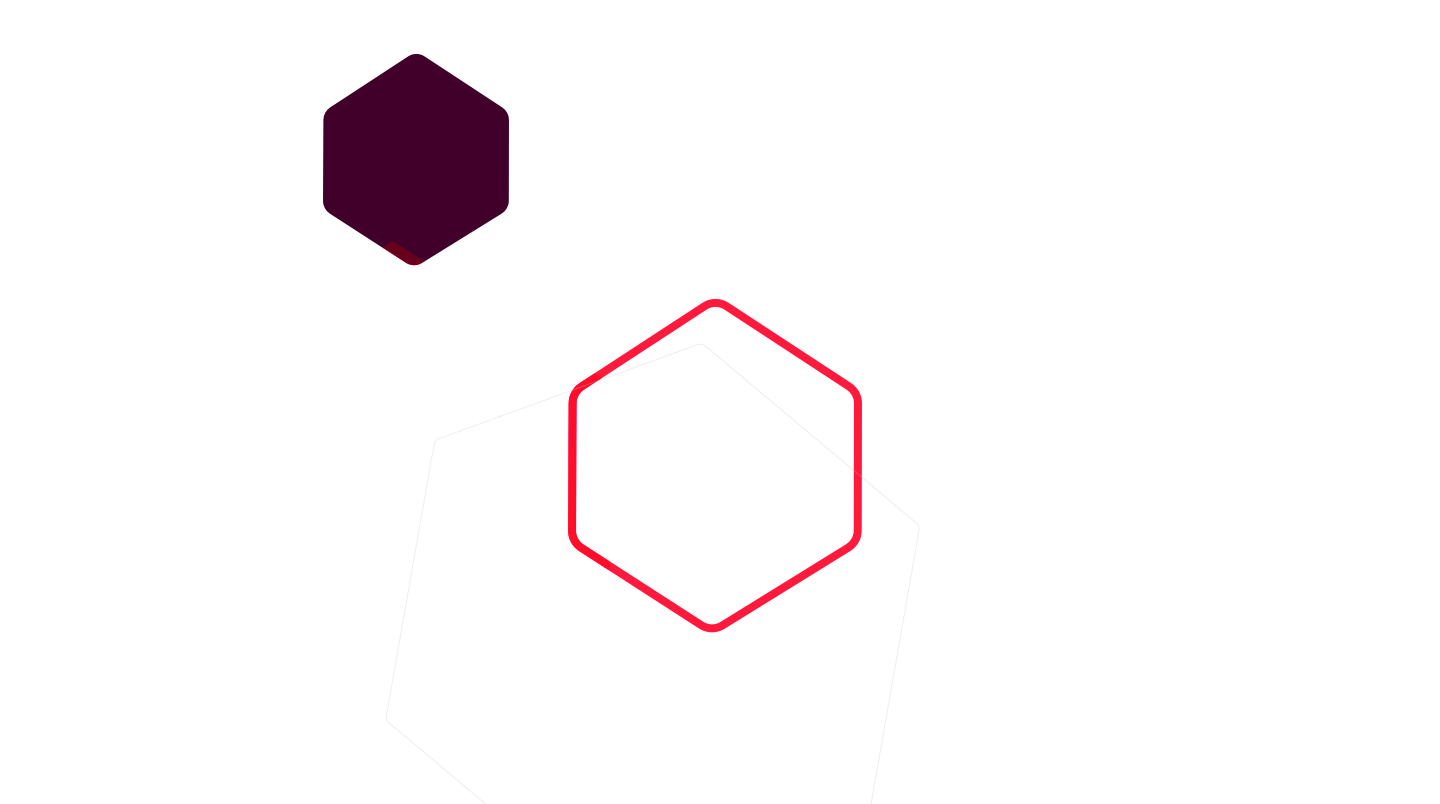
\includegraphics[width=.5\paperwidth]{graphics/title-bg.png}
    };

  \end{tikzpicture}

% Version history
\begin{versionhistory}
  \vhEntry{1.0}{August 2020}{Kai Michaelis}{Initial version}
\end{versionhistory}
\end{titlingpage}

\thispagestyle{empty}
\tableofcontents

\chapter{Introduction}
immune Guard is a remote attestation and firmware monitoring solution with the
goal of being

\begin{itemize}
  \item usable with off-the-shelf systems,
  \item scalable,
  \item easy to deploy, integrate and maintain.
\end{itemize}

Additionally to authenticating UEFI, boot loaders and OS kernel immune
Guard monitors platform components that are not part of conventional Measured
Boot implementations like microcode version, Intel BootGuard
configuration and running Management Engine clients. 

immune Guard is able to leverage a system's Trusted Computing Module to record
boot code and identify a particular platform by its manufacturer's certificate.
This allows immune Guard to detect changes to the platform remotely and secure
data even after the platform has been attacked successfully.

immune Guard is built to allow easy horizontal scaling and segmenting the
server fleet into independent, but centrally manageable domains. 

\section{Purpose}

immune Guard provides a secure computing substrate for server platforms. It
secures platform firmware from the first instruction executed after power on,
to the operating system bootloader. Aside from code immune Guard verifies
the platform's hardware security features like BootGuard, Management Engine and
PFR. 

immune Guard monitors the version and configuration of all security-relevant
firmware components like Intel ME and UEFI BIOS to allow administrators to find
outdated and vulnerable systems and patch them.

% token
% security report


%\todo{security life cycle}
%\footnote{ID.AM, ID.RA, PR.AC, PR.DS, PR.IP, PR.MA, PR.PT, DE.AE and DE.CM}

%\todo{malware detetion}

\section{Environment}

\subsection*{Attacker Model}

immune Guard provides correct platform quotes in the presence of a
persistent attacker. The attacker model of immune Guard allows an attacker
control over all code running on the platform, including most of the UEFI/BIOS on
the on-board flash. The attacker is also permitted to eavesdrop, change, delay
and replay all communication between the agent and the trust anchor as well as
the agent and the verifier. Under these conditions immune Guard prevents an
attacker to persist on the system across cold resets without being detected. 

In order to provide these security guarantees immune Guard assumes that the
Core Roots of Trust for Reporting and Measurement are not under the control of
the attacker. This means that the trust anchor and the initial measurement code
is unchanged. To protect the initial measurement code (i.e. the Core Root of
Trust for Measurement) working flash write protections or technologies like
Intel TXT or AMD SKINIT are required but be correctly set up.

immune Guard also assumes that the chain of trust remains unbroken and includes
userland applications using technologies like dm-verity and Linux IAM. If this
is not the case immune Guard can detect all changes to code that is
executed until the end of the chain of trust.

Users do not need to fully trust the immune Guard Verifier and Agent and can
check the freshness and correctness of all reports received from the trust
anchor. This \emph{Zero Trust} mode of operation allows administrators to
ensure that reports are not changed, removed, reused or delayed. See
Section~\ref{app:zero} for cryptographic details.

%\todo{drtm/oproms}
%
%\todo{smm/stm}
%
%\todo{changes to report}
%
%\todo{trust in bios vendors}
%
%\todo{security of verifiers and management node}


\subsection*{Operational Model}

The management interface serves as the single source of truth for all verifiers and pushes all configured devices and policies to all verifiers. Verifiers themselves receive quotes from devices, try to match them against the configured policies and issue tokens independently from the central management interface. The management interface regularly pulls the latest quotes from the verifiers to compute a global view of the fleet and issue alerts. The initial registration of a device is also handled by the management interface. See Figure~\ref{fig:arch} for an overview of all components and their data flow.

\begin{figure}[ht!]
  \centerfloat
  \begin{tikzpicture}
    \SetEdgeStyle[LineWidth=0.5pt]
    \SetVertexStyle[
      TextFont=\bfseries \scriptsize,
      MinSize=15pt,
      FillColor=none,
      LineColor=transparent]
    \SetDistanceScale{1.5}


    \Vertex[y=0,x=4.5,label=Management,Pseudo,size=1]{mng}

    \Vertex[y=-2,x=2.5,label=Verifier $\alpha$,Pseudo]{v1}
    \Vertex[y=-2,x=6.5,label=Verifier $\beta$,Pseudo]{v2}

    \Vertex[y=-4,x=1,label=Server 1,Pseudo]{s1}
    \Vertex[y=-4,x=2,label=$\cdots$,Pseudo]{}
    \Vertex[y=-4,x=3,label=Server $n$,Pseudo]{s4}
                    
    \Vertex[y=-4,x=6,label=Server $n+1$,Pseudo]{s5}
    \Vertex[y=-4,x=7,label=$\cdots$,Pseudo]{}
    \Vertex[y=-4,x=8,label=Server $m$,Pseudo]{s8}

    \Text[y=-2.5,x=5.8]{\tiny \rmfamily Push reports}
    \Text[y=-2.5,x=1.5]{\tiny \rmfamily Push reports}

    \Text[y=-0.5,x=2.9]{\tiny \rmfamily Pull summaries}
    \Text[y=-1.5,x=4]{\tiny \rmfamily Configuration}
    \Text[y=-0.5,x=6.5]{\tiny \rmfamily Registration}

    \Edge[Direct,bend=15](v1)(mng)
    \Edge[Direct,bend=15](v2)(mng)
    \Edge[Direct,bend=15](mng)(v1)
    \Edge[Direct,bend=15](mng)(v2)

    \Edge[Direct](s1)(v1)
    \Edge[Direct](s4)(v1)
                         
    \Edge[Direct](s5)(v2)
    \Edge[Direct](s8)(v2)

    \Edge[Direct,bend=-30](s8)(mng)

  \end{tikzpicture}
  \caption{The immune Guard component architecture. Arrows point in the direction of the flow of data.}
  \label{fig:arch}  
\end{figure}

\pagebreak

\subsection*{Hardware Requirements}

To reliably secure machines against sophisticated attackers immune
Guard requires a TPM 2.0 compatible trust anchor. immune Guard is tested
against the following trust anchors.

\begin{itemize}
  \item Infineon OPTIGA
  \item STMicroelectronics STSAFE
  \item Nuvoton SafeKeeper
  \item Intel Platform Trust Technology
  \item AMD SecureProcessor
\end{itemize}

If none of these are available immune Guard uses a software trust anchor. It
provides the same SRTM features as hardware trust anchors but is less secure.

%\todo{UEFI, if SGX TPM}

\section{Protected Platform Parts}
\subsection*{Firmware}

immune Guard records all boot code starting at the first instruction of the
initial boot block, the UEFI/BIOS firmware and OS boot loader. This includes
all DXE modules run as part of the platform bringup. 

In conjunction with a SecureBoot enabled UEFI it records executed PCI option
ROMs and signed UEFI applications.

\subsection*{CPU and Management Engine}

What sets immune Guard apart is that it monitors parts of the platform
configuration that is not protected by Secure Boot or Trusted Platform Modules.
immune Guard prepares a platform security report that is bound to the signed
measurements and is sent alongside. When verifying the measurements the security
report is verified using the security policy configured for the device. A token
is only issued if both the measurements and the security report pass.

The security policy includes the following platform properties.

\begin{itemize}
  \item Type, manufacturer and firmware version of the installed Trusted
    Platform Module.
  \item TPM passwords \texttt{ownerAuth} and \texttt{endorsememntAuth} are
    secure.
  \item Intel TXT was set up correctly. The TXT public configuration space
    indicates no error and no secrets in memory.
  \item Intel TXT, BootGuard and SGX security version numbers (SVNs).
  \item Keys provisioned in the  Intel BootGuard Key Manifest.
  \item Initial boot block DMA protections.
  \item CPU debug and BSP init bits.
  \item Intel BootGuard boot status.
  \item CPU and southbridge pre-production state.
  \item TPM event log of the UEFI/BIOS.
  \item Intel SGX flexible launch control status and key fingerprint.
  \item Version and running clients of the Intel Management Engine.
  \item Configuration of the SMI Transfer Monitor.
  \item AMD Secure Boot status.
  \item Intel Platform Firmware Resilience (PFR) provisioning and boot status.
  \item Secure Boot certificates and revocations.
\end{itemize}

\subsection*{PCI Devices}
PCI and PCI-Express devices pose a considerable risk to system integrity. They
are able to overwrite system memory using DMA transfers and can inject code
into the boot process using option ROMs~\footnote{These devices can be attested
and secured using the DICE~\cite{dice} and PICe Security~\cite{pciesec}
protocols. But, the low adoption rate of these standards forces us to choose
other means.}. immune Guard uses the UEFI SecureBoot standard to prevent rouge
PCI(-Express) devices from providing option ROMs of illegitimate origin. The
list of executed ROMs are part of the security report and thus can be limited
by a security policy.

\chapter{Components}
immune Guard consists of three components: verifier, agent and management
interface. The agent runs on each protected device and handles communication
between the trust anchor and the verifier. The verifier receives quotes from
the agents and issues cryptographic tokens to them. These can be used to
authenticate a protected device against third party services. The management
interface configures verifiers and receives their events. It also hosts both
the API endpoints as well as the web UI. The management interface is the
only component with a global view of the system.

\section{Verifier}
The verifier receives signed PCR values and security reports from protected
devices and matches them against the configured security policy. After
successful verification, the verifier generates and signs a new token. This
token is sent to the protected device. Aside from producing tokens the verifier
also provides a web API for validating them (c.f. Section~\ref{sec:validate}). 

Each verification attempt by an agent generates an event containing the
verification result and additional metadata. This event pulled by the mana
interface where they are accumulated to infer the current state of all
protected devices.

The verifier has a local database of all protected devices that can be
verified together with their security policy. The database is read by the
verifier and updated by the management interface.

Each verifier contains two certificates. One for authenticating all
communication with the management interface and one for signing tokens issued
to protected devices. Both certificates are certified by the management
interface as part of the verifier registration (c.f. Section~\ref{sec:reg}). 

The verifier listens on TCP port 443 for connections by agents and the
management interface. All other network access can be blocked.

\section{Agent}

The agent is a self-contained application that enrolls the protected device at
the management interface (c.f. Section~\ref{sec:enroll}), generates quotes
using the system's trust anchor and retrieves tokens from the verifier (c.f.
Section~\ref{sec:attest}).

The agent can run on-demand or as a service in the background. It keeps
only a limited state between invocations and can work on systems with no or
read-only file systems. The state consists of the keys and their certificates
generated as part of the enrollment process as well as the last token issued by
the verifier. Systems without persistent memory need to be re-enrolled after
each boot. 

\subsection*{Agent Permissions}

The agent needs to communicate with the system's trust anchor. In case
of a TPM 2.0 this means read/write access to the \texttt{/dev/tpm*} device
node. 

To compile a security report of the platform the agent also needs to
access

\begin{enumerate}
    \item \label{perm:txt} the public TXT/BG memory space,
    \item the eSPI controller,
    \item various machine specific registers,
    \item the Intel ME device,
    \item UEFI variables and
    \item \label{perm:flash} the on-board flash.
\end{enumerate}

To access~\ref{perm:txt} and~\ref{perm:flash} the agent needs either
read access to the \texttt{/dev/mem} device or must be able to load a
specialized kernel module that makes this data temporally accessible. If none of
these are possible the report will not include the status of TXT provisioning
and flash write protections.

Per default, the agent binary has the SUID bit set and is owned by the
\texttt{root} user. After reading all necessary data the agent drops all
privileges.

In terms of network access, the agent needs to connect to the verifier using TCP
port 443 to retrieve a security token. If the protected device needs to be
enrolled the agent needs access to the management interface via TCP port 80.
All other network access can be blocked.

\subsection*{Agent Kernel Module}

In order to access platform configuration data mapped into memory the agent
needs to read from physical addresses \texttt{0xFFFF0000} to \texttt{0xFFFFFFFF}
(memory mapped on-board flash) and \texttt{0xFED30000} to \texttt{0xFED40000}
(TXT public configuration space).

The classic way to read this data is through the \texttt{/dev/mem} device. For
security reasons, access to this device is limited or disabled on most Linux
distributions. On these platforms, the agent can load a specialized kernel
module that makes these memory ranges accessible. The module is licensed under
GPL2 and can be built using DKMS. The module gives user space applications
read-only access to the on-board flash contents and the TXT public
configuration space via \texttt{sysfs}.

\section{Management Interface}

The management interface is the central repository of all protected devices,
security policies and verifiers. It hosts the web UI and API for view, add,
delete and manipulate device metadata and security policies. The
management interface pulls events from verifiers and thus has a global
view of the fleet.

The management interface pulls updates from all registered Verifiers. These are
lists of received security reports and issued tokens. Thus, the management
interface knowns about all current and past tokens for each protected device
and can selectively revoke them.

The management interface also handles the public key infrastructure used to
issue certificates to verifiers, which in turn are used to sign tokens.
Consumers of tokens ask the management interface for the certificate hierarchy
used to sign these.

Devices are enrolled by adding their Endorsement key certificate fingerprint
to the management interfaces database. This information is subsequently pushed
to all verifiers. Removing devices from the fleet works the same way.

\subsection*{Alerting}

The management interface is responsible for alerting administrators about
unscheduled changes to devices. Modification of a device's firmware and
platform configuration results in failures to verify reports by one or more
Verifiers. These are collected by the management interface for correlation and
deduplication. Because the management interface has a global view of all changes
to the fleet it's able to detect false-positives like automatic, unscheduled
firmware updates. This information can be included in alerts to reduce the
mental load on administrators.

Alerts are delivered as emails and to Slack.

\subsection*{Backup}
The database of the management interface contains all enrolled devices and
security policies and  necessary to recover an immune Guard setup in case of a
catastrophic failure. Backing up the database using PostgreSQL provided
mechanisms suffices as a backup. Note that security reports that have not been
pulled from the Verifiers will be lost.

%\todo{PXE server}

\section{Operator Tool}

The operator tool is a command-line interface that can be used to perform
administrative tasks without using the web UI.  Additionally, the operator tool
can read platform information and query the trust anchor of the system it's
running on. The main task of the tool is to enroll new devices by extracting a
trust anchor's Endorsement key and current platform configuration. Both are
uploaded to the management interface as known-good values. The operator tool
can also be used to prepare firmware updates for fleets by creating a new
security policy based on the platform configuration of a single machine that
serves as a template for the rest of the fleets devices. The operator tool
can verify quotes independently of the management interface.

\chapter{Processes}

In the context of immune Guard, devices inhabit one of six states:
\emph{Unknown}, \emph{New}, \emph{Registered}, \emph{Trusted}, \emph{Modified}
or \emph{Expired}. Only devices in the Trusted state can be considered secure.
Processes are actions the Agent, Verifier and Management components of immune
Guard do to transition devices from one state to another. Actions have
prerequisites and can fail. If an action's prerequisites are not fulfilled or
the action fails the devices remain in their original state. See
Figure~\ref{fig:states} for an overview of what state transitions are possible.

\begin{figure}[ht!]
  \centerfloat
  \begin{tikzpicture}[->,>=stealth',shorten >=1pt,auto,node distance=3.3cm,
    initial text = ]
    \tikzstyle{every state}=[minimum size=1.5cm]

    \node[initial,state]      (unk)                           {\footnotesize Unknown};
    \node[state]              (new)      [above right of=unk] {\footnotesize New};
    \node[state]              (regd)     [right of=new]       {\footnotesize Registered};
    \node[state,circle split] (trusted)  [right of=regd]
      {\footnotesize Trusted \nodepart{lower} \footnotesize Modified};
    \node[state]              (expired)  [right of=trusted]   {\footnotesize{Expired}};

    \path (unk)     edge                    node {\footnotesize enroll}   (new)
          (new)     edge                    node {\footnotesize register} (regd)
          (regd)    edge                    node {\footnotesize attest}   (trusted)
          (trusted) edge [loop above]       node {\footnotesize attest}   (trusted)
          (trusted) edge [bend left]        node {\footnotesize timeout}  (expired)
          (expired) edge [bend left]        node {\footnotesize attest}   (trusted)
          (trusted) edge [dashed,bend left] node {\footnotesize revoke}   (unk)
          (expired) edge [dashed,bend left] node {\footnotesize revoke}   (unk)
          (new)     edge [dashed,bend left] node {\footnotesize revoke}   (unk)
          (regd)    edge [dashed,bend left] node {\footnotesize revoke}   (unk);
  \end{tikzpicture}
  \caption{States of protected devices (circles) and the possible state transitions between them (arrows).}
  \label{fig:states}  
\end{figure}

Devices start in the Unknown state in which immune Guard it not aware of the
device. Enrolling a device into immune Guard moves it to the New state. A New
device transitions to the Registered state by establishing a set of keys inside
the Protected Device's trust anchor. Now, devices can become Modified or
Trusted by sending a security report to a Verifier. If the report matches the
configured security policy of the device it becomes Trusted, otherwise it's
considered Modified. The state can potentially change with ever new report that
is sent. If the validitiy period of a report is over and no new report has been
received since the devices transitions to the Expired state. Devices that are
New, Registered, Modified, Trusted or Expired can be decommissioned which
removes them from immune Guard and thus back to the Unknown state.

The details and exact prerequisites of all immune Guard actions are described in
the remainder of this chapter.

\section{Enrollment}
\label{sec:enroll}

Before protected devices can be attested they must be made known to immune Guard,
a process called enrollment. Enrolling a device requires that its Endorsement Key
certificate's fingerprint is entered into the management interface database.
Optionally, a security policy can be associated with the device.

Endorsement Key certificate fingerprints can be received through an out of band
channel (e.g. a list emailed by the manufacturer) and entered either in the web
UI or by the operator tool. Alternatively, the Platform Certificate can be used
to enroll a device. The Platform Certificate includes the Endorsement Key
certificate as well as a reference to the expected PCR values. This allows
immune Guard to generate a security policy for the device.

If the Endorsement key certificate of the protected device is unknown the
enrollment process can be run as part of the registration (c.f.
Section~\ref{sec:reg}). This follows the Trust On First Use (TOFU) security
model which has weaker security guarantees but has less operational overhead.

After the device's Endorsement key certificates fingerprint is known to the
management interface the enrollment is done.

%\section{Provisioning}
%
%\todo{txt}

\section{Registration}
\label{sec:reg}

The registration process follows the enrollment and precedes the first
attestation. A protected device is registered by generating and certifying the
necessary keys for signing and encrypting the attestation evidence produced by
the trust anchor (c.f. Figure~\ref{fig:reg}). 

\begin{figure}[ht!]
  \centerfloat
  \begin{sequencediagram}
    \def\unitfactor{1}

    \newthread{dev}{Device}
    \newinst[2]{anc}{Trust anchor}
    \newinst[2]{mng}{Management Interface}

    \begin{call}{dev}{}{anc}{Public keys}
    \end{call}
    \begin{call}{dev}{EK, public keys}{mng}{\begin{minipage}{2cm}{Encrypted
    certificates}\end{minipage}}
      \begin{callself}{mng}{Verify keys}{}
      \end{callself}
    \end{call}
    \begin{call}{dev}{\begin{minipage}{2cm}{Encrypted
    certificates}\end{minipage}}{anc}{Certificate}
    \end{call}
  \end{sequencediagram}
  \caption{The immune Guard registration protocol.}
  \label{fig:reg}  
\end{figure}

immune Guard uses a hierarchy of three keys to do all cryptographic operations
on the device side (c.f. Figure~\ref{fig:hierarchy}). The Attestation Identity Key
(AIK) is used to sign the TPM 2.0 Quote that includes the measured PCR values,
the current TPM uptime, a verifier-provided nonce and a hash of the security
report send alongside. The Transport Key (TK) is used as a TLS client
certificate when connecting to the verifier. Both keys are generated under the
root key. TK and AIK are generated inside the trust anchor and never leave it
unencrypted. The exact parameters used for the keys can be found in
Appendix~\ref{app:keys} on page~\pageref{app:keys}.

\begin{figure}[ht!]
  \centerfloat
  \begin{tikzpicture}[edge from parent]
    \tikzstyle{edge from parent}=[->,draw]

    \node (device) {Device root key}
      child { node (tk) {Transport Key} }
      child [level distance=2.25cm, sibling distance=2.75cm] { node (aik)
      {Attestation Identity Key} };

    \node[xshift=2.75cm,right of=device] (ek) {Endorsement key};

    \node[above of=ek,yshift=1.5cm] (manu) {TPM manufacturer};

    \draw [->] (manu) -- (ek);

    \node (pki) [right of=ek,xshift=4cm] {Server root CA}
      child { node (tls)  {TLS certificate} };

    \draw [->] (pki) -- (aik);

    \node[anchor=south west, above left of=device,xshift=-0.8cm,yshift=0.5cm]
      {\small\textbf{Trust anchor}};
    \begin{pgfonlayer}{background}
      \draw [draw,dashed]
        ($(aik.south -| tk.west)+(-0.5cm,-0.5cm)$) rectangle ($(device.north -|
        ek.east)+(0.5cm,0.5cm)$);
   \end{pgfonlayer}
  \end{tikzpicture}
  \caption{The immune Guard key hierarchy. The trust anchor
  generates three keys for all cryptographic operations with the management
interface and the verifier. Additionally, the pre-provisioned Endorsement key is
used to identify the device.}
  \label{fig:hierarchy}
\end{figure}

The registration process is initiated the first time a protected device
attempts to attest itself by the verifier. The need for a registration is
detected by the lack of AIK or TK on the device. The device requests the trust
anchor to generate the needed keys and to output their public keys. The device
then sends the public keys of AIK and TK, evidence for their correct creation
and the Endorsement key certificate to the management interface. The management
interface will then verify that,

\begin{itemize}
  \item public keys of AIK and TK have the correct usage attributes and
    cryptographic properties,
  \item the creation evidence is liked to the keys and proves that the keys
    were generated inside the trust anchor and
  \item the Endorsement key certificate is valid and was signed by the trust
    anchor manufacturer.
\end{itemize}

If the Endorsement key certificate is unknown to the management interface (i.e.
the Endorsement key certificates fingerprint is not in the database), it is
automatically enrolled if this isn't disabled by the administrator. 

The management interface then issues certificates for AIK and TK signed by its
PKI. These certificates are encrypted using the Endorsement key. The device
receives both encrypted certificates, uses the trust anchor to decrypt them
(so-called Credential Activation) and saves them on disk. 

\section{Attestation}
\label{sec:attest}

The enrolled and registered devices can be attested at any time. The attestation
process is initiated by the device and illustrated in Figure~\ref{fig:attest}.

\begin{figure}[ht!]
  \centerfloat
   \begin{sequencediagram}
     \newthread{dev}{Device}
     \newinst[2]{anc}{Trust anchor}
     \newinst[2]{rel}{Relying party}
     \newinst[2]{ver}{Verifier}

     \begin{call}{dev}{}{anc}{Quote}
     \end{call}
     \begin{call}{dev}{Certificate, quote, report}{ver}{Token}
      \begin{callself}{ver}{Verify quote}{}
      \end{callself}
      \end{call}
     \begin{call}{dev}{Token}{rel}{}
     \end{call}
   \end{sequencediagram}
   \caption{The immune Guard attestation protocol.}
   \label{fig:attest} 
\end{figure}

First, the device creates a security report that summarises the unmeasured parts of the
platform configuration. Second, it connects to the verifier using TLS. The
device authenticates itself using the TK certificate issued as part of the
registration process. The verifier sends a nonce to the device. The device then
requests a signed set of measurements from the trust anchor. This signature also
includes the nonce and the fingerprint of the security report. The signature,
measurements, security report, AIK certificate and Endorsement key certificate
are sent to the verifier. Which in turn makes sure that,

\begin{itemize}
  \item the signature is valid and was produced by the sent AIK,
  \item the nonce signed with the measurements and security report is the one
    sent before,
  \item the AIK certificate is valid and was issued by the management interface
    PKI,
  \item the Endorsement key certificate is the same as mentioned on the AIK
    certificate,
  \item the Endorsement key certificate correspondents with an enrolled device,
  \item the measurements and the security report conform to the configured
    security policy, if one exists and
  \item the TK certificate used as TLS client certificate is valid, issued by
    the management interface PKI and correspondents to the Endorsement key
    certificate.
\end{itemize}

After all these checks pass the verifier issues a JSON Web Token (JWT) to the
device. The verifier will also send an event to the management interface that
the attestation was successful. The event includes the device Endorsement key
fingerprint, security report and measurements. The verifier keeps copies of a
fixed number of past events for each device in its database.

If one of the above checks fail the verifier signals an error to the device and
closes the connection. It sends an event to the management interface detailing
the error and its source.

\pagebreak

\section{Token Verification}
\label{sec:validate}

The JWT issued to attested devices is signed by the verifier that received the
device measurements. It proves that a particular device was successfully
attested in the past. Verifying the token can be done by every third party by
fetching the certificate used to sign the JWT from the issuing verifier and
checking the JWTs signature (c.f. Figure~\ref{fig:token}). The verifier that
issued the token can also produce the full measurements, security report and
nonce send by the device the JWT was issued to. For this, the verifier
implements an API that returns this information for each JWT on request.

\begin{figure}[ht!]
  \centerfloat
   \begin{sequencediagram}
     \newthread{dev}{Device}
     \newinst[2]{rel}{Relying party}
     \newinst[2]{ver}{Verifier}

     \begin{call}{dev}{Token}{rel}{\emph{Access granted}}
       \begin{call}{rel}{Token}{ver}{\begin{minipage}{2cm}{\raggedright Device
       identity and security status}\end{minipage}}
       \postlevel
       \postlevel
       \postlevel
     \end{call}
     \end{call}
   \end{sequencediagram}
   \caption{Using the immune Guard token for authentication.}
   \label{fig:token} 
\end{figure}

%\chapter{Usage}
%\section{Deployment and Maintenance}
%\section{Devices and Provisioning}
%\section{Security Policies}
%\section{Events and Audit Logs}
%\section{Relying Parties}

\begin{appendix}
\chapter{Cryptography}

\section{TPM 2.0 Key Parameters}
\label{app:keys}

To sign the attestation evidence and encrypt the communication between agent
and verifier, the trust anchor generates two asymmetric key pairs, Transport
key and Attestation Identity key. Both are generated under the root key.
Neither keys' private portion ever leaves the trust anchor unencrypted.

The transport and Attestation Identity keys are ECC key pairs over NIST curve
P-256 using ECDSA. The root key is an RSA key pair with a 2048 bit long public
modulus using PKCS\#1 v1.5. It encrypts the TK and AIK using AES-128 in CFB
mode when they are stored outside the trust anchor.

Their exact creation parameters are the following:

\begin{table}[htbp]
  \centerfloat
  \begin{tabular}{@{}p{4cm}*{3}{L{\dimexpr4cm\relax}}@{}}
    \toprule
    & Root & Transport & Attestation Identity \\
    \cmidrule{2-4}
    parentHandle & Endorsement Hierarchy & Root & Root \\
    inPublic.type & RSA & ECC & ECC \\
    \quad.nameAlg & SHA-256 & SHA-256 & SHA-256 \\
    \quad.objectAttributes & fixedTPM, fixedParent, userWithAuth,
    sensitiveDataOrigin, decrypt, restricted & fixedTPM, fixedParent,
    userWithAuth, sensitiveDataOrigin, sign & fixedTPM, fixedParent,
    userWithAuth, sensitiveDataOrigin, sign, restricted \\
    \quad.parameters.scheme & RSA / AES-128 / CFB & ECDSA / SHA-256 & ECDSA /
    SHA-256 \\
    \quad.parameters.keyBits & 2048 & N/A & N/A \\
    \quad.parameters.curveID & N/A & NIST P-256 & NIST P-256 \\
    outsideInfo & \texttt{IMMUNE GUARD ROOT KEY} & \texttt{IMMUNE GUARD TRANSPORT KEY} & \texttt{IMMUNE GUARD ATTESTATION IDENTITY KEY} \\
    \bottomrule
  \end{tabular}
  \caption{Detailed key parameters.}
  \label{fig:keys} 
\end{table}

As part of the registration process, the management interface certifies TK and
AIK by issuing X.509v3 certificates for both. These are encrypted using the
public part of the trust anchors Endorsement key. The Endorsement key is a 2048
bit RSA key pair on most TPM 2.0 devices.

\pagebreak

\section{Zero Trust Quotes}
\label{app:zero}

immune Guard has the option to use a externally provided random value (nonce) as
an additional input into the TPM 2.0 Quote operation. When this Zero Trust
feature is enabled immune Guard will also "chain" quotes together by combining
the previous quote with the nonce. This allows users to verify that they are
not served slate quotes and that quotes were generated in the advertised order.
See Algorithm~\ref{alg:zero} for details.

\begin{algorithm}
  \begin{algorithmic}[1]
    \Require $L:\text{Length of a TPM 2.0 nonce in bytes.}$
    \Require $I:\text{Static context string.}$
    \Require $S:\text{Customer and device dependent context string.}$
    \Require $seed:\text{Customer provided random value.}$

    \Procedure{Attest}{$seed$}
      \State $q_0 \gets \emptyset$
      \State $i \gets 1$
      
      \Loop
        \Comment{Start attesting the device}
        \State $prk_i \gets \Call{HKDF-Extract}{S, seed || q_{i-1}}$\Comment{Combine the previous Quote with seed}
        \State $n_i \gets \Call{HKDF-Expand}{prk_i, I , L}$\Comment{Generate a new nonce}
        \State $q_i \gets \Call{TPM4\_Quote}{\ldots, n_i}$\Comment{Request a Quote}
        \State $i \gets i+1$
      \EndLoop 
    \EndProcedure
  \end{algorithmic}
  \caption{Zero trust attestation.}
  \label{alg:zero}
\end{algorithm}

\bibliographystyle{unsrt}
\bibliography{bibtex}

%\section{Key Management}
%\section{Credential Activation}
%\section{Quoting}

\end{appendix}
\end{document}
